\documentclass[tikz,border=10pt]{standalone}
\usepackage{tikz}
\usetikzlibrary{arrows.meta,calc,positioning}

\tikzset{
  card/.style={draw=blue!70!black, rounded corners=4pt, line width=1.2pt, minimum width=4.6cm, minimum height=1.2cm, align=center, text width=4.1cm},
  note/.style={draw=orange!85!black, rounded corners=4pt, line width=1.2pt, minimum width=12.8cm, minimum height=1.1cm, align=center, text width=12.1cm},
  flow/.style={-{Stealth[length=3mm]}, line width=1.2pt, draw=black!70}
}

\begin{document}
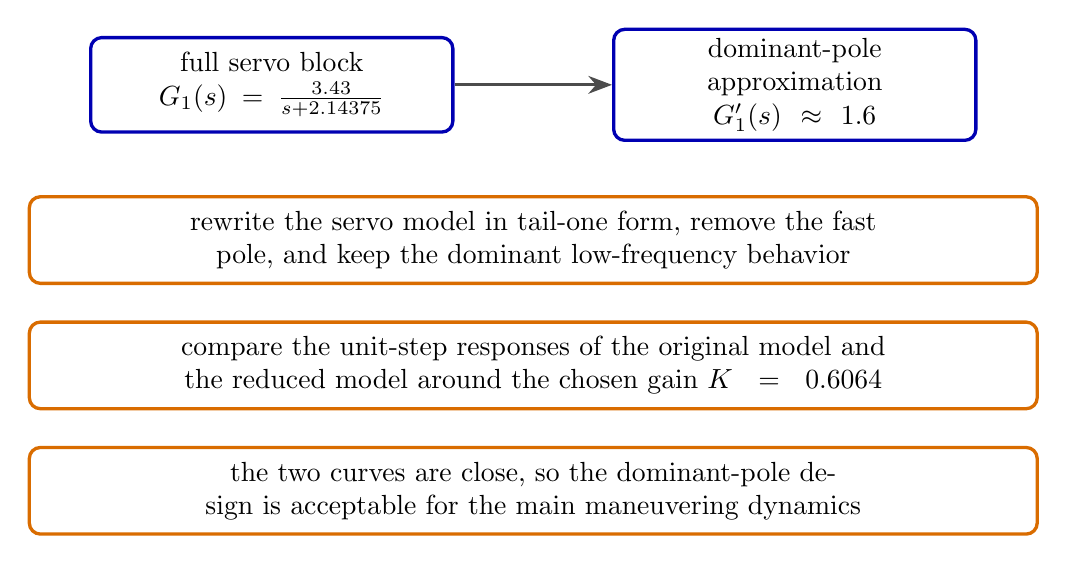
\begin{tikzpicture}[node distance=1.2cm]
  \node[card] (full) {full servo block\\$G_1(s)=\frac{3.43}{s+2.14375}$};
  \node[card, right=2.0cm of full] (approx) {dominant-pole approximation\\$G_1'(s)\approx 1.6$};
  \node[note, below=1.4cm of $(full)!0.5!(approx)$] (n1) {rewrite the servo model in tail-one form, remove the fast pole, and keep the dominant low-frequency behavior};
  \node[note, below=0.45cm of n1] (n2) {compare the unit-step responses of the original model and the reduced model around the chosen gain $K=0.6064$};
  \node[note, below=0.45cm of n2] (n3) {the two curves are close, so the dominant-pole design is acceptable for the main maneuvering dynamics};

  \draw[flow] (full) -- (approx);
\end{tikzpicture}
\end{document}
